\documentclass[simplex.tex]{subfiles}
% NO NEED TO INPUT PREAMBLES HERE
% packages are inherited; you can compile this on its own
\begin{document}
\subsection{Non-Parametric Shape Clustering}
%% Jan
We developed a prototype algorithm for 2-dimensional shape clustering, which
is invariant under affine transformations. This employs the procrustes
distance between two objects, which requires feature extraction to obtain
landmark points; see Fig.~\ref{fig:nonpar} for an example. 
We intend to apply a variant of this method to analyze neural synapses,
since we have such datasets from our collaborators. However, to this particular
dataset, the preprocessing techniques may be highly sophisticated, and a new
metric to compare different objects may be necessary. Moreover, these shapes are
3-dimensional. We are currently working on this project
with our collaborators, extending our existing  techniques to this 
particular dataset.

We also started working on a related, and more general, project.
We intend to develop non-parametric clustering algorithms with statistical
guarantees. We will use an energy-statistics based approach. Given
two datasets $X$ and $Y$, there is an energy function $\mathcal{E}(X,Y)$
test statistic which allows us to infer if $X$ and $Y$ have the same
distribution. Our results thus far suggest that this can be written
as a quadratic optimization problem
with quadratic constraints: 
\begin{equation}
\max_{x,z\in \mathbb{R}^N} x^T \Delta z \qquad \mbox{s.t. $x_i^2=1$, $x+z = 0$}
\end{equation}
where $\Delta$ is a dissimilarity data matrix.
There is not enough literature on
this interesting problem, so this will very likely lead to new methods which
can have interesting applications, in particular to neuroscience datasets.

\begin{figure}[h!]
\begin{cframed}
\centering
\begin{subfigure}[t]{0.45\textwidth}
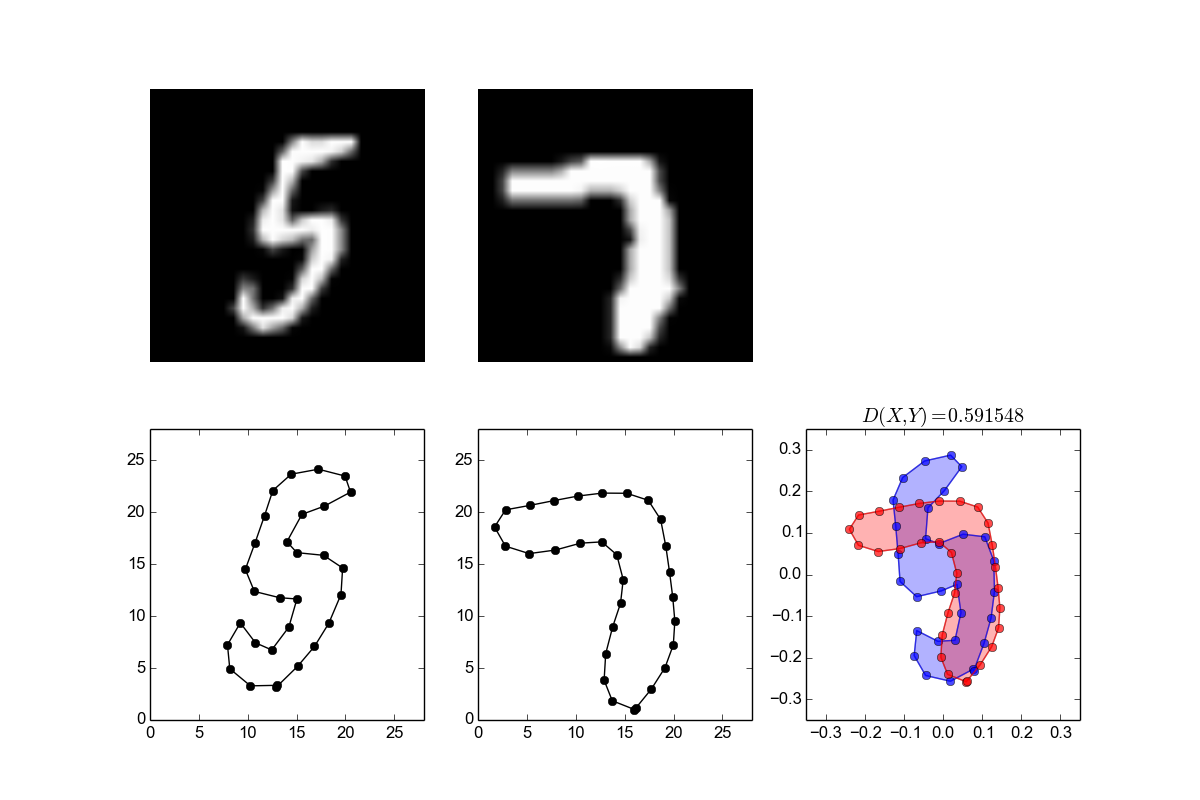
\includegraphics[width=\textwidth]{../../figs/nonpar57.png}
\label{fig:nonpar57}
\caption{
  MNIST digits with extracted landmarks and alignment.
  }
\end{subfigure}
\begin{subfigure}[t]{0.45\textwidth}
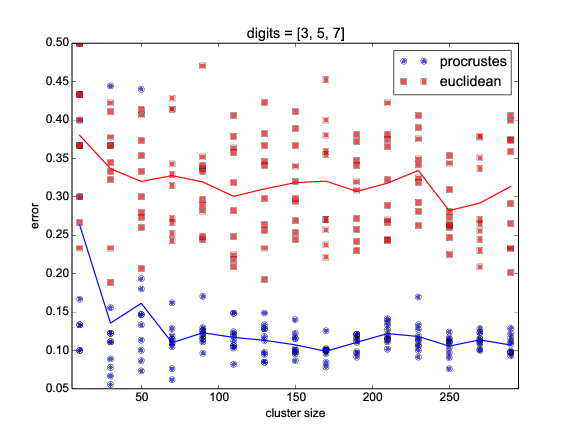
\includegraphics[width=\textwidth]{../../figs/nonPar357.png}
\label{fig:nonpar357}
\caption{
Classification error against the size of each
cluster (the three classes have the same number of points) is
shown in blue. The red line is standard
K-means with Euclidean distance for comparison.}
\end{subfigure}
\caption{
  MNIST handwritten digits and classification error results.
}
\label{fig:nonpar}
\end{cframed}
\end{figure}
\clearpage

%%% Feb
We have been mostly focused on developing 
non-parametric clustering methods.
To this purpose, we are exploring ideas from energy statistics,
which is non-parametric,
robust, and rotational invariant, thus it incorporates the main ingredients
that we are looking for. The main difficulty is to formulate an 
algorithm based on this, i.e. to identify the correct test 
statistic, or to formulate it as a feasible optimization problem.
Consider $K$-Means clustering problem which is 
$
\min_{\{\mathcal{C}_k\}} 
\sum_{k=1}^K \sum_{x \in \mathcal{C}_k} \| x - \mu_k  \|^2,
$
where $\mathcal{C}_k$ is the $k$th cluster and $\mu_k$ the mean of its points.
We showed that this problem is equivalent to
\begin{equation}
\max_{G} \textnormal{Tr}\left( G^T K G \right) \qquad 
\mbox{s.t. \, $G \ge 0$, $G^T G=I$, $G G^T e_1 = e_1$}.
\end{equation}
where $e_1 = (1,1,\dotsc,1)^T$.
This is a Quadratically Constrained Quadratic Problem (QCQP), which is usually 
NP-hard.
Analogously, consider the energy function 
$\mathcal{E}(F,G) = 2\mathbb{E} \| X - Y\| - \mathbb{E}\| X - X'\| - \mathbb{E}
\| Y - Y'\|$ between $X,X' \sim F$ and $Y,Y' \sim G$. We showed that this can
be written as $\mathcal{E}(A,B) = e_1^T \Delta e_1 $, where $\Delta$ is a
dissimilarity 
matrix between the two sets of data points 
$A \stackrel{iid}{\sim} F$ 
and $B \stackrel{iid}{\sim} G$.
Consequently, a simple two-class clustering problem would be
\begin{equation}
\max_{x,z\in \mathbb{R}^N} x^T \Delta z \qquad 
\mbox{s.t. $x_i^2=1$, $x+z = 0$},
\end{equation}
which is also a QCQP problem. We are currently investigating this problem and
trying to generalize it correctly for more classes.
A simple check of the energy function as a test statistic 
is shown in Fig.~\ref{fig:nonpar}. 
Under the null $F = G$, 
$T$ converges to a quadratic form of normally distributed random variables. This
seems to be the case in the first (blue) histogram, while it is definitely not
the case in the other (red and green) histograms. 
For the blue histogram a single test gives
$T \approx 0.32$ (small), for the red
histogram $T \approx 4000 $ (large), and for the green 
histogram $T \approx 105$ (large), with
only a few points. Thus, energy statistics based approach is 
able to distinguish between
different distributions, even when the clusters have the same mean, which is a
property that $K$-Means cannot resolve.

%
\begin{figure}[h!]
\begin{cframed}
\centering
%\begin{subfigure}[t]{0.45\textwidth}
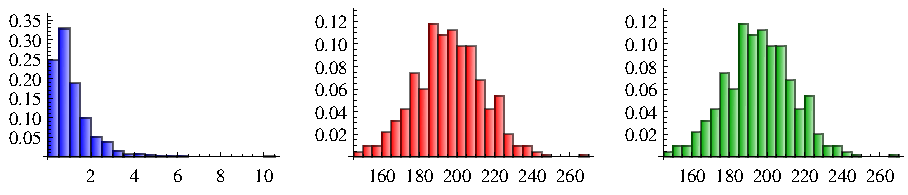
\includegraphics[width=\textwidth]{../../figs/energy_hists.pdf}
%\label{fig:nonpar57}
\caption{
Distribution of test statistic 
$T\equiv\tfrac{n m }{n+m}\mathcal{E}(A,B)$ 
for an ensamble obtained from two distributions:
$A \stackrel{iid}{\sim} \mathcal{N}(\mu_A,\sigma_A^2)$ and
$B \stackrel{iid}{\sim} \mathcal{N}(\mu_B, \sigma_B^2)$, where
$|A|=n$ and $|B|=m$.
Blue histogram: $\mu_A = \mu_B = 0$ and $\sigma_A = \sigma_B = 1$;
Red histogram: $\mu_A = - \mu_B = 1$ and $\sigma_A = \sigma_B = 1$;
Green histogram: $\mu_A = \mu_B = 0$, $\sigma_A = 1$ and $\sigma_B = 1.5$.
}
\label{fig:nonpar}
\end{cframed}
\end{figure}
%
\clearpage

%% March
Energy statistics provides a nonparametric test for equality of distributions.
It is rotational invariant which is a highly desirable quality
for clustering. For a two-class problem, $X,X' \sim \mu$ and 
$Y,Y' \sim \nu$, where $\mu,\nu$ are CDFs, it reads
\begin{equation}\label{eq:energy}
\mathcal{E}(X,Y) = 2\mathbb{E} \| X - Y \|
- \mathbb{E} \| X - X' \| - \mathbb{E} \| Y - Y'\|.
\end{equation}
We are developing a clustering framework based on \ref{eq:energy}.
Our criteria is that $\mathcal{E}$ should be a maximum when data points are
correctly classified.
%
It is possible to show that there is a map from the data space of $X,Y$
to the probability space of $\mu,\nu$ which is a Hilbert space whose
inner product  can be obtained from a kernel 
function related to \ref{eq:energy}, 
$\langle \mu, \nu \rangle
= k(x,y)$.
This enables us to formulate our clustering problem as follows:
\begin{equation}\label{eq:opt}
\textnormal{max} \left\{ \textnormal{Tr} L^{1/2} Z^T K Z L^{1/2} \right\}
\quad
\textnormal{s.t.} \quad 
\, Z_{ij}\in\{0,1\}, \sum_i Z_{ij} = N_j, \sum_j Z_{ij}=1,
Z^T Z = L^{-1}
\end{equation}
where $N_j$ is the number of elements in the $j$th cluster,
$L^{-1}=\textnormal{diag}(N_1,\dotsc,N_k)$, and $K$ is the Gram 
matrix obtained
from the kernel. Let $\mathcal{X}$ be the pooled data matrix. If we
replace $K \to \mathcal{X}^T \mathcal{X}$ we recover the well-known
$k$-means problem, which in this formulation is related
to spectral clustering and normalized cuts. Problem
\ref{eq:opt} is 
NP-hard and a numerical implementation is prohibitive even
for small data sets. We are investigating how to 
solve \ref{eq:opt} in
a feasible way. As an evidence that \ref{eq:opt} is the correct optimization
problem, and more importantly, it illustrates the power behind our proposal,
in Fig.~\ref{fig:plots} we generate data and plot the objective in 
\ref{eq:opt} versus $n$, where $n$ is the number of points randomly shuffled
from one class to the other. Therefore, for $n=0$ the function must be a
maximum. We do this for the kernel related to \ref{eq:energy} (blue dots)
and compare with the kernel related to $k$-means (red dots).
Clearly, \ref{eq:opt} based on \ref{eq:energy} is able to distinguish
between different cluster even for complex data sets that are
not linearly separable. Moreover, in our formulation
there are no free-parameters in the kernel.

\begin{figure}[h!]
\begin{cframed}
\centering
\begin{minipage}{0.49\textwidth}
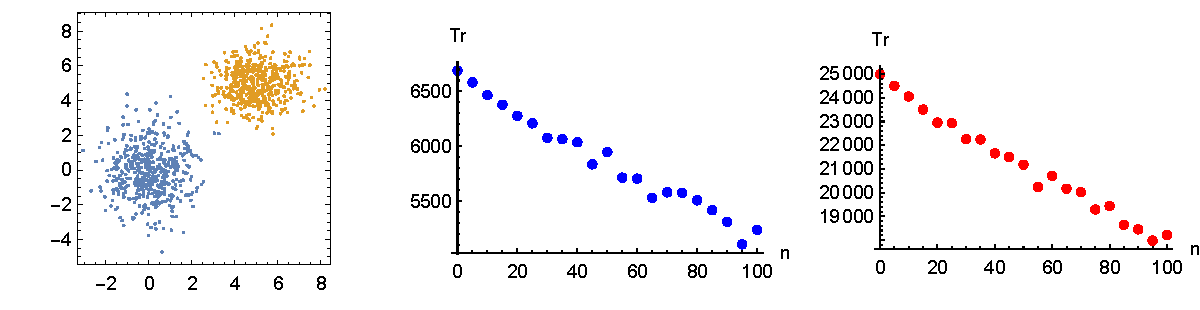
\includegraphics[scale=.37]{../../figs/plot1.pdf}
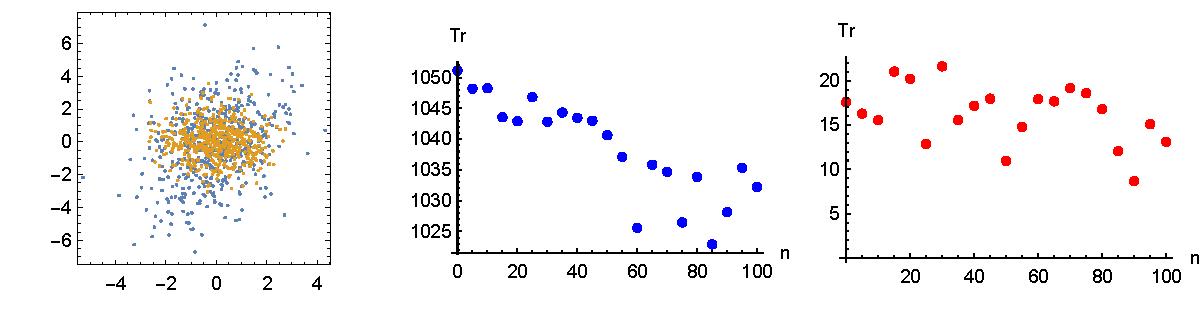
\includegraphics[scale=.37]{../../figs/plot2.pdf}
\end{minipage}
\begin{minipage}{0.49\textwidth}
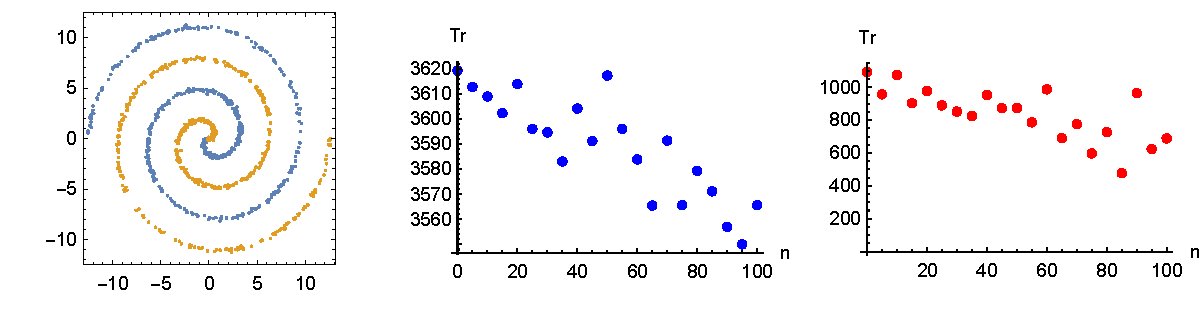
\includegraphics[scale=.37]{../../figs/plot3.pdf}
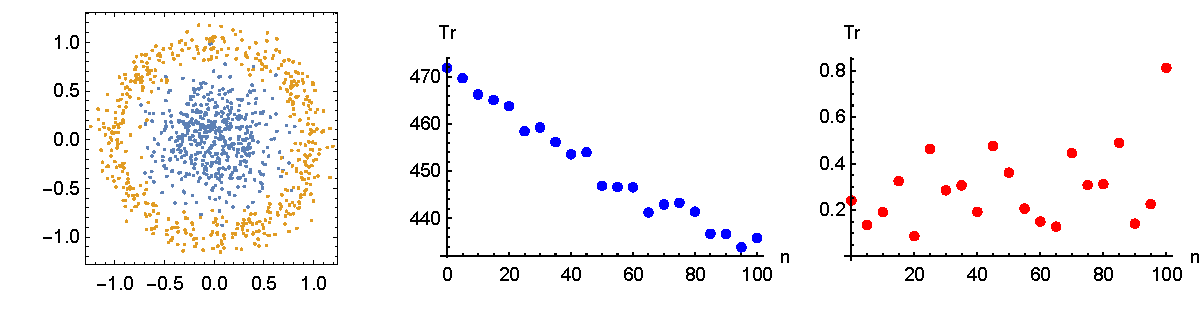
\includegraphics[scale=.37]{../../figs/plot4.pdf}
\end{minipage}
\caption{
Two dimensional datasets and the objective function
in \ref{eq:opt} as a function of $n$, where $n$ is the number of shuffled
points from its correct class to the wrong class. Blue dots
are for \ref{eq:energy} and red dots for $k$-means. A good function must
be monotonically decreasing. We can clearly see that \ref{eq:energy} is
way more powerful than $k$-means.
}
\label{fig:plots}
\end{cframed}
\end{figure}
\clearpage
\end{document}
